\documentclass{article}

\usepackage[solutions]{xrcise}

\begin{document}
\sheet[2012]{Ersttermin (Rarey)}

\begin{exercise}{Multiple Choice}
  Bei allen Multiple-Choice Fragen ist genau ein Kreuz zu setzen. Sollte mehr als ein Kreuz gesetzt sein, wird die Teilaufgabe mit 0 Punkten gewertet.
  \begin{enumerate}
    \item Gegeben sind die Funktionen \[
            n^2 \quad n! \quad n^{2n} \quad \sqrt{3} \quad \log n
          \] Welche der folgenden Aussagen gilt?
          \begin{itemize}
            \item[$\square$] Alle Funktionen sind polynomiell.
            \item[$\square$] $n!$ ist die am stärksten wachsende Funktion
            \item[$\square$] $\sqrt{3} n = \bigO(\log(n))$
            \item[$\square$] $n^2 + o(n^2) = \Theta(n^2)$
          \end{itemize}
    \item Seien $f(n), g(n)$ Funktionen. Weiter sei $h$ definiert durch $h(n) = \max(f(n), g(n))$. Gilt dann
          \begin{itemize}
            \item[$\square$] $h(n) = \bigO(f(n))$
            \item[$\square$] $h(n) = \bigO(f(n) + g(n))$
            \item[$\square$] $h(n) = \omega(f(n) + g(n))$
            \item[$\square$] $h(n) = \bigO(f(n) - g(n))$
          \end{itemize}
    \item Beschreiben Sie die Datenstruktur Schlange, die sich durch die folgende Sequenz von Operationen ergibt:\par
          \begin{quote}\textalgo{enqueue(15), rear(), enqueue(7), enqueue(8), dequeue(), enqueue(9), dequeue(), head(), enqueue(10)}\end{quote}
    \item Wir betrachten einen Baum $T$ mit Höhe $h$ (die Wurzel hat die Höhe 0) und $n$ Knoten. Die inneren Knoten von $T$ haben maximal drei Kinder. Welche der folgenden Aussagen ist wahr?
          \begin{itemize}
            \item[$\square$] $h$ ist immer $\log_3(n)$
            \item[$\square$] $T$ hat mindestens $n$ Kanten
            \item[$\square$] $T$ hat immer mehr Blätter als innere Knoten
            \item[$\square$] $T$ hat mindestens $n - 3h$ innere Knoten.
          \end{itemize}
    \item Sei $G = (V,E)$ ein zusammenhängender, ungerichteter Graph mit der Kantengewichtsfunktion $w$. Angenommen $w(e) = c, c$ konstant, für alle Kanten, welche Laufzeit lässt sich dann zur Berechnung des minimalen Spannbaumes in $G$ erreichen?
          \begin{itemize}
            \item[$\square$] $\bigO(|V| \log |E|)$
            \item[$\square$] $\bigO(|V| + |E|)$
            \item[$\square$] $\bigO(|E| \log |V|)$
            \item[$\square$] $\bigO(|V|^2)$
          \end{itemize}
    \item Fügen Sie den Wert 12 in die folgende Hashtabelle mit offener Addressierung und linearer Sondierung ein. Als Hashfunktion wird $h(x) = x \mod 7$ benutzt.
          \begin{center}
            \begin{tabular}{|c|c|c|c|c|c|c|c|}
              \hline
              0 & 1 & 2 & 3 & 4 & 5 & 6  \\
              \hline
              \hline
                & 5 & 9 &   &   & 5 & 13 \\
              \hline
            \end{tabular}
          \end{center}
    \item Führen Sie eine Linksrotation auf den Knoten $a$ aus.\begin{figure}
  \centering
  \begin{tikzpicture}[auto, on grid, node distance=1.5cm, treenode/.style={circle, draw}]
    \node [treenode] (e) {e};
    \node [treenode, below left=1cm and 2cmof e] (a) {\textbf{a}};
    \node [treenode, below right=1cm and 2cm of e] (g) {g};
    \node [treenode, below right=of a] (c) {c};
    \node [treenode, below left=of g] (f) {f};
    \node [treenode, below right=of g] (h) {h};
    \node [treenode, below right=of c] (d) {d};
    \node [treenode, below left=of c] (b) {b};

    \draw (e) -- (a) -- (c) -- (b);
    \draw (c) -- (d);
    \draw (e) -- (g) -- (f);
    \draw (g) -- (h);
  \end{tikzpicture}
  \caption{Tree before rotation}\label{fig:treerotate}
\end{figure}
    \item Seien $L, L' \in P$. Welche der folgenden Aussagen ist falsch?
          \begin{itemize}
            \item[$\square$] Wenn $L \in NP$ gilt, dann folgt $P = NP$
            \item[$\square$] $\forall L'' \in NPC:L \leq_p L''$
            \item[$\square$] $L \cap L' \in P$
            \item[$\square$] $L \cup L' \in P$
          \end{itemize}
    \item Welches ist die untere Schranke für die Anzahl der Vergleichsoperationen bei vergleichsbasierten Sortieralgorithmen?
          \begin{itemize}
            \item[$\square$] $\Omega(n)$
            \item[$\square$] $\Omega(\log(n))$
            \item[$\square$] $\Omega(n \log(n))$
            \item[$\square$] $\Omega(n^2)$
          \end{itemize}
    \item In einem minimalen Spannbaum eines Graphen mit $n$ Knoten
          \begin{itemize}
            \item[$\square$] kann die Kante mit dem höchsten Gewicht enthalten sein
            \item[$\square$] darf die Kante mit dem kleinsten Gewicht nicht enthalten sein
            \item[$\square$] können mehr als $n - 1$ Kanten enthalten sein
            \item[$\square$] muss die Summe der Kantengewichte durch 2 teilbar sein
          \end{itemize}
    \item In einem Rot-Schwarz-Baum gilt (ohne Betrachtung der Wächter) für alle roten Knoten $r$
          \begin{itemize}
            \item[$\square$] der Vor-Vorgänger von $r$ ist rot, falls der Elter von $r$ nicht die Wurzel ist
            \item[$\square$] der Bruder Knoten von $r$ ist rot
            \item[$\square$] Wenn $r$ kein Blatt ist, dann hat $r$ zwei Kinder
            \item[$\square$] der Onkel von $r$ ist schwarz
          \end{itemize}
  \end{enumerate}
  \begin{solution}
    \begin{enumerate}
      \item \xmark, \xmark, \xmark, \checkmark
      \item \xmark, \checkmark, \xmark, \xmark
      \item $[8, 9, 10]$
      \item \xmark, \xmark, \checkmark, \xmark
      \item \xmark, \xmark, \checkmark, \xmark
      \item $12$ an Position $0$ nach $3$ Versuchen
      \item Folgender Baum ergibt sich nach Left-Rotation: \begin{figure}
  \centering
  \begin{tikzpicture}[auto, on grid, node distance=1.5cm, treenode/.style={circle, draw}]
    \node [treenode] (e) {e};
    \node [treenode, below left=1cm and 2cmof e] (c) {c};
    \node [treenode, below right=1cm and 2cm of e] (g) {g};
    \node [treenode, below left=of c] (a) {\textbf{a}};
    \node [treenode, below right=of c] (d) {d};
    \node [treenode, below left=of g] (f) {f};
    \node [treenode, below right=of g] (h) {h};
    \node [treenode, below right=of c] (d) {d};
    \node [treenode, below right=of a] (b) {b};

    \draw (e) -- (c) -- (a) -- (b);
    \draw (c) -- (d);
    \draw (e) -- (g) -- (f);
    \draw (g) -- (h);
  \end{tikzpicture}
  \caption{Tree after rotation}\label{fig:treerotated}
\end{figure}
      \item \xmark, \xmark, \xmark, \checkmark
      \item \xmark, \xmark, \checkmark, \xmark
      \item \checkmark, \xmark, \xmark, \xmark
      \item \xmark, \xmark, \checkmark, \xmark
    \end{enumerate}
  \end{solution}
\end{exercise}

\begin{exercise}{Algorithmenanalyse}
  \begin{enumerate}
    \item Betrachten Sie die folgenden Code-Segmente. Geben Sie für jedes Segment eine möglichst dichte Schranke für die asymptotische Laufzeit im O-Kalkül in Abhängigkeit von $N$, bzw. $N = \text{length}[A]$ an. Bei rekursiven Algorithmen formulieren Sie zuvor die Rekurrenzgleichung. (Teil-Arrays werden immer als Kopie übergeben, das Kopieren kostet keine Zeit.)
          \begin{enumerate}
            \item $\bigO(?)$
                  \begin{alg}\signed{alg1}{}{\empty}
                    \For{$i \gets 0$ \KwTo $N$}{
                      \For{$j \gets N$ \textbf{downto} $1$}{
                        \textbf{do} $sum \gets sum + 1$\;
                      }
                    }
                  \end{alg}
            \item $\bigO(?)$
                  \begin{alg}\signed{alg2}{}{\empty}
                    \For{$i \gets 1$ \KwTo N}{
                      \textbf{do} $j \gets N$\;
                      \While{$j > 1$}{
                        \textbf{do} $sum \gets sum + j$\;
                        \textbf{do} $j \gets j/2$\;
                      }
                    }
                  \end{alg}
            \item $\bigO(?)$
                  \begin{alg}\signed{alg3}{}{\empty}
                    \While{$N > 1$}{
                      \For{$j \gets 1$ \KwTo $N$}{
                        \textbf{do} $sum \gets sum + j$\;
                      }
                      $N \gets N/2$\;
                    }
                  \end{alg}
            \item $T(n)=\{?$ and $\bigO(?)$
                  \begin{alg}\signed{alg4}{A}{\empty}
                    $middle \gets \text{length}[A]/2$\;
                    $sum \gets sum + A[1]$\;
                    \If{$\text{length}[A] > 2$}{
                      \call{alg4}{A[1 \dots middle]}\;
                      \call{alg4}{A[middle + 1 \dots \text{length}[A]]}\;
                    }
                  \end{alg}
            \item $T(n)=\{?$ and $\bigO(?)$
                  \begin{alg}\signed{alg5}{A}{\empty}
                    \For{$i \gets 1$ \KwTo $\text{length}[A]$}{
                      \textbf{do} $sum \gets sum + A[i]^2$\;
                    }
                    \If{$\text{length}[A] > 3$}{
                      \call{alg5}{A[1 \dots \text{length}[A]/3]}\;
                      \call{alg5}{A[\text{length}[A]/3 \dots 2 \cdot \text{length}[A]/3]}\;
                      \call{alg5}{A[2 \cdot \text{length}[A]/3 \dots \text{length}[A]]}\;
                    }
                  \end{alg}
            \item $T(n)=\{?$ and $\bigO(?)$
                  \begin{alg}\signed{alg6}{A}{\empty}
                    \For{$i \gets 1$ \KwTo $\text{length}[A]$}{
                      \textbf{do} $sum \gets sum + A[i]$\;
                    }
                    \If{$\text{length}[A] > 1$}{
                      \call{alg6}{A[1 \dots \text{length}[A] - 2]}\;
                    }
                  \end{alg}
            \item $T(n)=\{?$ and $\bigO(?)$
                  \begin{alg}\signed{alg7}{A}{\empty}
                    \textbf{do} $sum \gets sum + 1$\;
                    \If{$\text{length}[A] > 1$}{
                      \call{alg7}{A[1 \dots \text{length}[A] - 2]}\;
                      \call{alg7}{A[2 \dots \text{length}[A] - 1]}\;
                    }
                  \end{alg}
          \end{enumerate}
    \item Bestimmen Sie die asymptotische Laufzeit des folgenden Algorithmus mit der Substitutionsmethode, geben Sie Ihren Lösungsweg an:
          \begin{alg}\signed{alg8}{A, N, n}{\empty}
            \If{$n \geq 2$}{
              \For{$i \gets 1$ \KwTo $n$}{
                \textbf{do} $\text{swap}(A[i], A[r])$\;
                \call{alg8}{A, N, n - 1}\;
                \textbf{do} $\text{swap}(A[r], A[i])$\;
              }
            }
            \Else{
              $sum \gets 0$\;
              \For{$i \gets 1$ \KwTo $N$}{
                \textbf{do} $s \gets s + A[i]$\;
              }
            }
          \end{alg}
          Die Funktion wird aufgerufen mit: $\text{alg8}(A, \text{length}[A], \text{length}[A])$
          \hint{Verwenden Sie folgende Notation: $[n]_i = n \cdot (n - 1) \cdot \ldots \cdot (n - i)$}
          \hint{Verwenden Sie die Abschätzung $[n]_i \leq n!$, wenn dies nicht zu einer Erhöhung der Laufzeitschranke im O-Kalkül führt.}
  \end{enumerate}

  \begin{solution}
    \begin{enumerate}
      \item \begin{enumerate}
              \item $\bigO(N^2)$
              \item $\bigO(N \log N)$
              \item $\bigO(N)$
              \item $T(n)= \begin{cases}
                        1                  & \text{if } n \leq 2 \\
                        2 \cdot T(n/2) + 1 & \text{sonst}
                      \end{cases}$ und $\bigO(N)$
              \item $T(n)= \begin{cases}
                        1                  & \text{if } n \leq 3 \\
                        3 \cdot T(n/3) + n & \text{sonst}
                      \end{cases}$ und $\bigO(N \log N)$
              \item $T(n)= \begin{cases}
                        1          & \text{if } n \leq 1 \\
                        T(n-2) + n & \text{sonst}
                      \end{cases}$ und $\bigO(N^2)$
              \item $T(n)= \begin{cases}
                        1                  & \text{if } n \leq 1 \\
                        2 \cdot T(n-1) + 1 & \text{sonst}
                      \end{cases}$ und $\bigO(N)$
            \end{enumerate}
      \item $T(n)=\begin{cases}
                n              & \text{if } n < 2 \\
                n \cdot T(n-1) & \text{sonst}
              \end{cases}$ und $\bigO(n!)$
    \end{enumerate}
  \end{solution}
\end{exercise}

\begin{exercise}{Quicksort}
  \begin{enumerate}
    \item
          Gegeben sei die bekannte Partitionsfunktion aus dem Quicksort-Algorithmus
          \begin{alg}
  \signed{Partition}{A, l, r}{\empty}
  \params{$l$ - linkes Blockende, $r$ - rechtes Blockende, $A$ - Array}{\empty}
  $i \gets l - 1$\;
  \For{$j \gets l$ \KwTo $r - 1$}{
    \If{$A[j] \leq A[r]$}{
      $i \gets i + 1$\;
      swap $A[i], A[j]$\;
    }
  }
  swap $A[i + 1], A[r]$\;
  \KwRet{$(i + 1)$}\;
\end{alg}
          Dabei gehen wir in dieser Aufgabe von Arrays mit 0-basiertem Index aus. Sie befinden sich in Zeile 4 der Partition-Funktion mit $l = 0, r = 6$ und $j = 3, i = 0$. Werten Sie alle Schritte bis zum Erreichen der Zeile 8 aus. Protokollieren Sie den Speicherzustand jeweils beim Erreichen der Zeile 3 und der Zeile 7.
          \begin{itemize}
            \item[Zeile 4] $A: 3, 8, 6, 4, 6, 4, 5$ \hfill $j = 3, i = 0$
            \item[Zeile 4] $A:\ ?$ \hfill $j = 4, i =\ ?$
            \item[Zeile 4] $A:\ ?$ \hfill $j = 5, i =\ ?$
            \item[Zeile 8] $A:\ ?$ \hfill $j = 5, i =\ ?$
          \end{itemize}
    \item Ist Quicksort mit der obigen Partition Funktion ein stabiles Sortierverfahren? Begründen Sie Ihre Antwort und zeigen Sie entweder, dass Partition stabil ist oder schlagen Sie eine Modifikation von Quicksort vor, welche diesen stabilisiert.
    \item Gegeben sei ein Array der Länge $N$, welches ausschließlich Elemente aus der Menge $0,1,2$ enthält. Entwerfen Sie einen Algorithmus, der die Elemente in $\bigO(n)$ Zeit sortiert. Der Algorithmus soll vergleichs-/austauschbasiert und in-place arbeiten, was bedeutet, dass er maximal $\bigO(1)$ zusätzlichen Speicher nutzen darf. Skizzieren Sie Ihre Idee mit Pseudo-Code und einem beschreibenden Text.
  \end{enumerate}

  \begin{solution}
    \begin{enumerate}
      \item
            \begin{itemize}
              \item[Zeile 4] $A: 3, 8, 6, 4, 6, 4, 5$ \hfill $j = 3, i = 0$
              \item[Zeile 4] $A: 3, 4, 6, 8, 6, 4, 5$ \hfill $j = 4, i = 1$
              \item[Zeile 4] $A: 3, 4, 6, 8, 6, 4, 5$ \hfill $j = 5, i = 1$
              \item[Zeile 8] $A: 3, 4, 4, 8, 6, 6, 5$ \hfill $j = 5, i = 2$
            \end{itemize}
      \item Quicksort mit der gegebenen Partition ist stabil. Wenn ein Element dem Pivot entspricht, wird es ebenfalls getauscht. Das Pivotelement wird zuletzt hinter diesen anderen platziert. Somit bleibt die Reihenfolge von gleichen Elementen erhalten und Quicksort sortiert stabil.
      \item Der Algorithmus zählt die Anzahl der Elemente $0,1,2$ und schreibt diese in das Array zurück. Der Algorithmus benötigt $\bigO(n)$ Zeit und $\bigO(1)$ zusätzlichen Speicher.\begin{alg}\signed{sort}{A}{\empty}
  $c_0, c_1, c_2 \gets 0$\;
  \For{$i \gets 0$ \KwTo $\text{length}[A]$}{
    \Switch{$A[i]$}{
      \lCase{0}{$c_0 \gets c_0 + 1$}
      \lCase{1}{$c_1 \gets c_1 + 1$}
      \lCase{2}{$c_2 \gets c_2 + 1$}
    }
  }
  \lFor{$i \gets 0$ \KwTo $c_0 - 1$}{$A[i] \gets 0$}
  \lFor{$i \gets c_0$ \KwTo $c_0 + c_1 - 1$}{$A[i] \gets 1$}
  \lFor{$i \gets c_0 + c_1$ \KwTo $c_0 + c_1 + c_2 - 1$}{$A[i] \gets 2$}
\end{alg}
    \end{enumerate}
  \end{solution}
\end{exercise}

\begin{exercise}{Minimaler Spannbaum}
  \begin{figure}
  \centering

  \caption{A graph}\label{fig:mstgraphrarey}
\end{figure}
  \begin{enumerate}
    \item Zeichnen Sie in den oben angegebenen Graphen einen minimalen Spannbaum ein. Ist dieser Spannbaum eindeutig? Begründen Sie Ihre Antwort.
    \item Gegeben sei ein Graph $G = (V,E)$. Entwerfen Sie einen rekursiven Algorithmus \texttt{Label(V, E, u, ’label’)}, der einen Knoten $u$ und alle von $u$ aus erreichbaren Knoten mit der Markierung ’label’ versieht. Der Algorithmus soll die Laufzeit $\bigO(|V| + |E|)$ haben. Beschreiben Sie Ihren Algorithmus und geben Sie Pseudo-Code für die Funktion \texttt{Label} an.
    \item In einem Graphen $G = (V,E)$ mit Kantengewichten bezeichnen wir eine Kante $e$ eines minimalen Spannbaums $T$ als kritisch, wenn das Entfernen von $e$ das Gewicht des minimalen Spannbaums in $G$ vergrößert. Entwickeln Sie einen Algorithmus, der in $\bigO(|V| + |E|)$ Zeit entscheidet, ob $e$ kritisch ist. Nutzen Sie dabei die Funktion \texttt{Label} aus der vorausgehenden Aufgabe als Hilfsfunktion. Beschreiben Sie kurz Ihren Lösungsweg und geben Sie den Algorithmus im Pseudo-Code an. Argumentieren Sie außerdem in wenigen Stichpunkten, warum Ihr Algorithmus korrekt ist.
  \end{enumerate}

  \begin{solution}
    \begin{enumerate}
      \item \begin{figure}
  \centering
  \begin{tikzpicture}[auto,on grid, node distance=2cm, main node/.style={circle,draw,fill=black}]
    \node [main node] (a) {};
    \node [main node,right=of a] (b) {};
    \node [main node,right=of b] (c) {};
    \node [main node,below=of c] (d) {};
    \node [main node,below=of d] (e) {};
    \node [main node,left=of e] (f) {};
    \node [main node,left=of f] (g) {};
    \node [main node,above=of g] (h) {};
    \node [main node,above=of h] (i) {};

    \path (a) edge node {4} (h);
    \path (b) edge node {3} (h);
    \path (c) edge node {7} (d);
    \path (d) edge node {1} (e);
    \path (d) edge node {1} (h);
    \path (f) edge node {2} (g);
    \path (g) edge node {2} (h);

  \end{tikzpicture}
  \caption{An MST}\label{fig:mstgraphrareysolution}
\end{figure} Der MST ist nicht eindeutig, da gleiche Kantengewichte zugelassen sind.
      \item Führe eine DFS aus und markiere alle besuchten Knoten mit ’label’. Der Algorithmus hat die Laufzeit $\bigO(|V| + |E|$).
            \begin{alg}

\end{alg}
      \item Ehrlich gesagt komme ich hier nicht voran. % TODO: Lösungsweg und Algorithmus
    \end{enumerate}
  \end{solution}
\end{exercise}

\begin{exercise}{Graphen}
  \begin{figure}
  \centering
  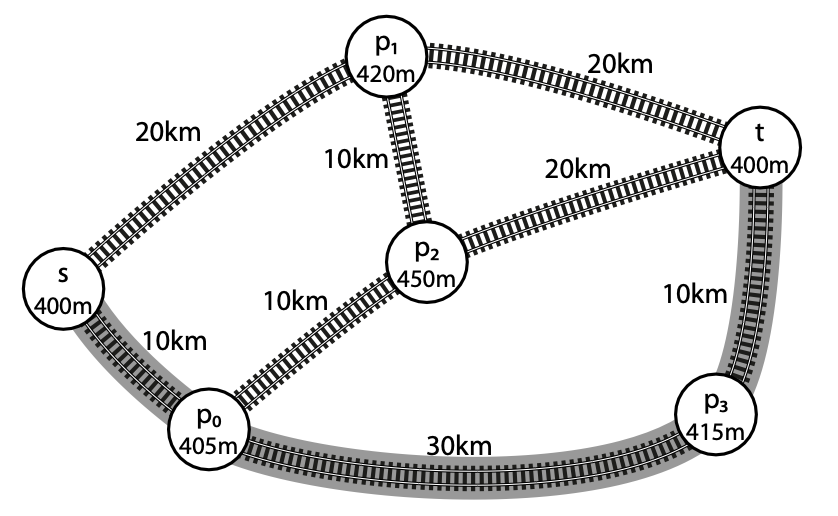
\includegraphics{res/trains.png}
  \caption{Train line graph.}\label{fig:trains}
\end{figure}
  Eine neue Eisenbahnlinie soll gebaut werden und Sie wurden mit ihrer Planung beauftragt. Zur Verfügung steht Ihnen eine topographische Landkarte mit möglichen Streckenverlaufspunkten $p_i$. Auf der Karte sind die Distanzen in km zwischen den Punkten eingetragen sowie die Höhe der Streckenverlaufspunkte über Normalnull in Metern. Ihr Auftrag lautet, eine Bahnlinie zwischen zwei gegebenen Punkten $s, t$ zu bestimmen, auf welcher ein Zug möglichst wenig Energie umsetzt. Die umgesetzte Energie bestimmt sich dabei wie folgt:
  \begin{itemize}
    \item 1 Energieeinheit pro km Strecke
    \item 2 Energieeinheiten pro Anstieg um einen Meter
    \item -1 Energieeinheit pro Abfall um einen Meter
  \end{itemize}
  \begin{enumerate}
    \item Wieviel Energie wird auf dem in der Karte grau markierten Pfad von $s$ nach $t$ (über $p_0$ und $p_3$) umgesetzt? Gibt es einen energetisch günstigeren Pfad?
    \item Modellieren Sie das Problem so, dass Sie einen aus der Vorlesung bekannten Algorithmus benutzen können. Beschreiben Sie Ihre Modellierung und nennen Sie den Algorithmus, der angewendet werden kann.
    \item Durch Einsatz einer moderneren Lok ändert sich der Energieverbrauch pro Anstieg um einen Meter auf 1 Energieeinheit. Zeigen Sie, dass nun im allgemeinen Fall für zwei beliebige Knoten $s, t$ gilt: der Pfad von $s$ nach $t$ mit den wenigsten Streckenkilometern entspricht dem Pfad mit dem minimalem Energieverbrauch.
  \end{enumerate}

  \begin{solution}
    \begin{enumerate}
      \item Der Pfad von $s$ nach $t$ über $p_0$ und $p_3$ hat eine Länge von 50 km und einen Energieverbrauch von $50+2\cdot 15-15=65$ bzw. 60 Energieeinheiten (je nachdem ob Energie für Gesamtstrecke oder für jede Teilstrecke berechnet wird). Ein energetisch günstigerer Pfad ist der Pfad von $s$ nach $t$ über $p_1$ mit einer Länge von 40km und einem Energieverbrauch von $40+2\cdot 40-20=60$ Energieeinheiten (nur falls für jede Teilstrecke der Energiebverbrauch einzeln berechnet wird).
      \item Das Problem kann als kürzester Pfad in einem Graphen modelliert werden, wobei die Kantengewichte die Energieverbrauchsfunktion repräsentieren. Der Algorithmus von Dijkstra kann zur Lösung des Problems verwendet werden.
      \item Der Pfad von $s$ nach $t$ mit den wenigsten Streckenkilometern entspricht dem Pfad mit dem minimalem Energieverbrauch, da sich der Aufstieg und Abstieg schlussendlich ausgleichen (da der letztendliche Höhenunterschied nicht durch den Pfad verändert wird).
    \end{enumerate}
  \end{solution}
\end{exercise}

\begin{exercise}{NP-Vollständigkeit}
  Paul hat einen Kasten mit $N$ Bauklötzen, die Klötze $k_i$ haben jeweils die Maße $b_i, t_i$ und $h_i$ (Breite / Tiefe / Höhe). Paul fragt sich, ob er mit den Klötzen einen Turm bauen kann, der exakt genau so hoch ist wie sein Schreibtisch (Schreibtischhöhe $H$). Dabei kann jeder Klotz beliebig gestapelt werden.
  \begin{enumerate}
    \item Zeigen Sie durch Reduktion auf ein Ihnen bekanntes Problem, dass Pauls Problem NP-vollständig ist.
    \item Entwickeln Sie ein Backtracking-Algorithmus zur Lösung von Pauls Problem. Skizzieren Sie in wenigen Stichpunkten Ihren Lösungsweg und geben Sie den Algorithmus in Pseudo-Code an.
    \item Paul möchte nun den höchsten Turm bauen, der noch unter seinen Schreibtisch passt. Geben Sie Schranken an, die verwendet werden können um den Backtracking-Algorithmus in einen Branch\&Bound Algorithmus umzuwandeln.
    \item Paul stellt beim Vermessen seiner $N$ Klötze fest, dass alle eine Grundfläche von $1 \times 1$ cm haben und außerdem entweder $6, 3$ oder $2$ cm hoch sind. Ist Pauls Problem unter dieser Randbedingung noch NP-vollständig? Begründen Sie Ihre Antwort.
  \end{enumerate}

  \begin{solution}
    \begin{enumerate}
      \item 3-SAT lässt sich auf Pauls Problem reduzieren, indem jede Klausel einen Würfel darstellt und die Höhe des Schreibtisches die Anzahl der Klauseln repräsentiert. Pauls Problem ist somit NP-vollständig.
      \item Für jeden Klotz überprüfen ob er auf den bisher gebauten Turm passt und rekursiv alle Möglichkeiten durchgehen.\par
            Wenn die Höhe des Turms der des Schreibtisches entspricht, den Turm zurückgeben.
            \begin{alg}

\end{alg}
      \item Der Algorithmus kann durch die Verwendung von Schranken in einen Branch\&Bound Algorithmus umgewandelt werden. Eine untere Schranke ist die Höhe des höchste bereits gebaute Turm, welcher nicht größer ist als die Höhe des Schreibtisches abzgl. dem höchsten noch nicht verwendeten Klotz. Eine obere Schranke ist (offensichtlich) die Höhe des Schreibtisches.
      \item Pauls Problem ist unter dieser Randbedingung nicht mehr NP-vollständig, da die Anzahl der möglichen Klötze und die Anzahl der möglichen Höhen begrenzt ist. Das Problem kann in polynomieller Zeit gelöst werden: \begin{itemize}
              \item lege Klötze seitlich auf den Turm (Höhe 1cm) bis alle verbraucht sind, gebe zurück falls Höhe des Schreibtisches erreicht
              \item drehe 2er Klötze (Höhe 2cm) bis alle gedreht sind, falls Höhe des Schreibtisches erreicht, gebe zurück
              \item drehe 3er Klötze (Höhe 3cm) bis alle gedreht sind, falls Höhe des Schreibtisches erreicht, gebe zurück
              \item drehe 6er Klötze (Höhe 6cm) bis alle gedreht sind, falls Höhe des Schreibtisches erreicht, gebe zurück
              \item falls Schreibtischehöhe nicht erreicht, gebe zurück, dass kein Turm gebaut werden kann
            \end{itemize} Der Algorithmus hat die Laufzeit $\bigO(N)$.
    \end{enumerate}
  \end{solution}
\end{exercise}

\end{document}